\chapter{EVE-ng}
\label{chap:eve_ng}

EVE-ng je virtuálne sieťové laboratórium skladajúcej sa zo serverovej časti postavenej na platforme Linux a klientskej časti, ktorú tvorí webová aplikácia, ako je už spomenuté v kapitole \ref{chap:nastroje_pre_siet_virt} v časti \ref{chap:virt_lab_eve_ng}. V tejto kapitole bude opísaný proces nasadzovania EVE-ng servera do sieťovej infraštruktúry katedry: jeho inštalácie, následnej úpravy a základnej administrácie EVE-ng servera. Všetky kroky sú podrobne opísané v návodoch na priloženom CD v adresári \emph{eve-ng}.

{\huge TODO - serverová časť je realizovaná ako tzv. LAMP server - vysvetliť, čo je kde a ako použité}

Po inštalácii servera je potrebné do určitej miery upraviť aj konfiguráciu klientských počítačov, ktoré budú EVE-ng server používať. Úpravám na klientskej strane sa venujem v bode \ref{item:vzdialeny_pristup} v časti \ref{chap:vytvorenie_topo_eve-ng} - \nameref{chap:vytvorenie_topo_eve-ng}.




\section{Inštalácia}

EVE-ng bol inštalovaný a testovaný na dvoch platformách:

\begin{itemize}[noitemsep]
    \item VMware Workstation Player
    \item Fyzický server
\end{itemize}

Parametre VMware virtuálneho stroja a fyzického servera sú uvedené v tabuľke \ref{tab:server_parameters}. V oboch prípadoch bol EVE-ng server nasadený do DMZ zóny, preto v riadku \emph{IP adresa} uvádzam len posledný oktet ich IPv4 adries, keďže IP adresa DMZ siete je na katedre známa.

\begin{longtabu} to \textwidth {| X[5.0,cm] | X[5.0,cm] | X[5.0,cm] |}
\caption{Parametre EVE-ng serverov}
\label{tab:server_parameters} \\
\hline
    \textbf{Parametre \textbackslash~ Server} & \textbf{VMware} & \textbf{Fyzický server} \\
\hline
    \textbf{CPU} & 16 & 8 \\
\hline
    \textbf{Operačná pamäť (GB)} & 16 & 48 \\
\hline
    \textbf{EVE-ng verzia} & 2.0.3-80 & 2.0.3-86 \\
\hline
    \textbf{IP adresa} & .49 & .50 \\
\hline
\end{longtabu}

\noindent
Uvedené tvrdenia platia pre EVE-ng vo vydaní \emph{Community Edition} vo verzii 2.0.3-86.

\noindent
Postup inštalácie EVE-ng servera môžeme zhrnúť do týchto krokov:

\begin{enumerate}[noitemsep]
    \item Vytvorenie vzdialenej pracovnej plochy
    \item Inštalácia Ubuntu Server 16.03
    \item Konfigurácia Ubuntu Server
    \item Inštalácia EVE-ng do Ubuntu Server
    \item Konfigurácia EVE-ng servera
\end{enumerate}

\noindent   
Konfigurácia EVE-ng servera zahŕňala:

\begin{enumerate}[noitemsep]
    \item Obnovenie súborov a adresárov
    \begin{itemize}[noitemsep]
        \item Skripty
        \item Zariadenia
        \item Databázy
    \end{itemize}
    \item Automatizácia zálohovania
    \item Pridanie Cisco IOL/IOU licencie
    \item Zabezpečenie servera
    \begin{itemize}[noitemsep]
        \item Systém
        \item SSH
        \item Webový server
    \end{itemize}
    \item Úprava šablón
    \item Úprava zdrojových kódov
\end{enumerate}

Inštalačný proces pre obe platformy, virtuálnu aj fyzickú, bol takmer zhodný, líšil sa iba v úvodných krokoch. Pri inštalácii pre VMware bolo totiž potrebné na server, na ktorom bol VMware nainštalovaný pridať VNC prístup a doplniť grafické prostredie, aby bolo možné ovládať grafické rozhranie VMware Player a spustiť virtuálny stroj. Pre VMware Player to bolo jediným riešením, ako vytvoriť virtuálny EVE-ng server.

Rozdielov medzi oboma inštaláciami je niekoľko. Prvým z nich je už spomenutá verzia. VMware inštalácia má nižšiu verziu, pretože bola nainštalovaná skôr. VMware inštalácia slúžila na prvotné odladenie a pilotné nasadenie do vyučovania. Nebola v nej vykonaná takmer žiadna dodatočná konfigurácia, okrem importu zariadení pre topológie.

Následná inštalácia EVE-ng na fyzický server vychádzala zo skúseností získaných z inštalácie EVE-ng do VMware prostredia. EVE-ng fyzický server bol odladený a do veľkej miery testovaný. Testovaniu zariadení v EVE-ng sa venujem v kapitole \ref{chap:testovanie_zariadeni} - \nameref{chap:testovanie_zariadeni}.

Nasadzovaniu jednotlivých EVE-ng serverov sa venujem v kapitole \ref{chap:nasadenie_do_vyucovania} - \nameref{chap:nasadenie_do_vyucovania}. Obnovovanie súborov a adresárov môžeme preskočiť, ak predtým ešte nebola vytvorená záloha príslušným zálohovacím skriptom. Zálohovaniu sa venujem v časti \ref{chap:zalohovanie} - \nameref{chap:zalohovanie}.

Pridanie Cisco IOL/IOU licencie je dôležitým krokom, bez ktorého by sme neboli schopní spúšťať Cisco IOL/IOU zariadenia. Význam týchto zariadení bude vysvetlený v kapitole \ref{chap:testovanie_technologii} - \nameref{chap:testovanie_technologii}.

Zabezpečenie servera spočívalo hlavne v zabezpečení operačného systému, SSH prístupu a webového servera.

Zabezpečenie operačného systému obsahovalo vytvorenie štandardného používateľského konta so \emph{sudo} oprávneniami. Ten sa bude používať namiesto \emph{root} používateľa, čím bude zaistená vyššia bezpečnosť pri používaní systému.

Zabezpečenie SSH prístupu zahŕňalo v zablokovanie \emph{root} používateľa, explicitné definovanie povolených používateľov a skupín, vygenerovanie SSH kľúčov a vypnutie autentifikácie heslom. Autentifikácia SSH kľúčmi má aj tú výhodu, že oproti autentifikácii heslom nie je nutné zadávať heslo, čím odpadá aj nutnosť pamätať si ho. Každý počítač, ktorý by chcel EVE-ng server používať, by si musel svoj verejný SSH kľúč nahrať na server k danému používateľskému účtu. Rozhodli sme sa ale, že pre obidva servery bude ponechaná autentifikácia heslom.

Zabezpečenie webového servera Apache sa skladalo z vygenerovania SSL certifikátu a aktivácie protokolu HTTPS a presmerovania požiadaviek z HTTP na protokol HTTPS. Webový server však nie je zabezpečený na ani jednom serveri, pretože bolo potrebné odchytávať komunikáciu a nezašifrované vymieňané správy medzi klientom a EVE-ng serverom, pre potreby rozširovania funkcii v EVE-ng, ktorým sa venujem v časti \ref{chap:eve_ng_uprava_zdroj_kodov} - \nameref{chap:eve_ng_uprava_zdroj_kodov}.

Na serveri bola bola vykonaná aj úprava šablón, aby používateľ pri vytváraní topológie nemusel premýšľať nad technickými parametrami zariadenia, ktoré do topológie pridáva, ale na vyučovanú problematiku. Tak sa vytváranie topológii aj samotné vyučovanie stane plynulejším. Každé zariadenie, ktoré je možné do topológie pridať, si totiž načíta svoje technické parametre zo súboru zvaného šablóna. V šablóne môže byť pre zariadenie definovaný napr. počet pridelených jadier CPU, maximálne množstvo alokovateľnej operačnej pamäte, spúšťacie parametre zariadenia a pod. Úpravy šablón boli vykonané na základe testovania vybraných zariadení, ktoré opisujem v kapitole \ref{chap:testovanie_zariadeni_benchmark} - \nameref{chap:testovanie_zariadeni_benchmark}.




\section{Úprava nástroja EVE-ng}
\label{chap:eve_ng_uprava_zdroj_kodov}

EVE-ng muselo byť upravené aj v zdrojových kódoch, aby sa nástroj dal použiť aj vo vyučovaní. Nižšie sú uvedené úspešne vykonané zmeny.




\subsection{Metodika}

Na to, aby sme mohli odhadnúť, ktoré časti nástroja EVE-ng treba upraviť, sme použili nástroje \emph{Wireshark} a \emph{grep}.

Nástroj Wireshark slúžil na odchytávanie vymieňaných správ prostredníctvom REST API. Keďže webový server nebol zašifrovaný a používal HTTP protokol, mohli sme skúmať tieto správy v nezašifrovanom texte. Následne sme hľadali číselný kód správy v súboroch vo webovom adresári EVE-ng. To nám umožnilo spresniť odhad na tie časti zdrojového kódu, ktorých zmena by s veľkou pravdepodobnosťou mohla vyriešiť daný problém.




\subsection{Sprístupnenie používateľských rolí}
\label{chap:eve_ng_pouzivatelske_role}

V EVE-ng Community Edition je pre používateľov dostupná iba jedna používateľská rola \mbox{\emph{admin}}, čiže administrátor. Je to tak preto, lebo \emph{Community} verzia je určená pre osobné použitie, kde sa nepredpokladá viac používateľov, než je používateľ sám. Takéto správanie však nie je vhodné pre nasadenie do vyučovacieho procesu.

Odchytili sme preto správy pri úprave ľubovoľného používateľa. Zistili sme, že sa o.i. posiela aj správa \\
\texttt{Successfully listed user roles (60041)}. Po vyhľadaní výskytu kódu tejto správy v súboroch webového adresára sa ukázalo, že sa vyskytuje aj v súbore \\
\texttt{/opt/unetlab/html/includes/functions.php}.

Na sprístupnenie ďalších používateľských rolí, \emph{editor} - učiteľ a \emph{user} - používateľ resp. študent, bolo potrebné ich odkomentovať z funkcie \texttt{listRoles} v spomenutom súbore.

To vo web rozhraní sprístupnilo v dialógovom okne na vytvorenie a úpravu používateľa ďalšie používateľské role (obrázok \ref{obr:eve_ng_pouzivatelia_dialog}).

\begin{figure}
    \centering
    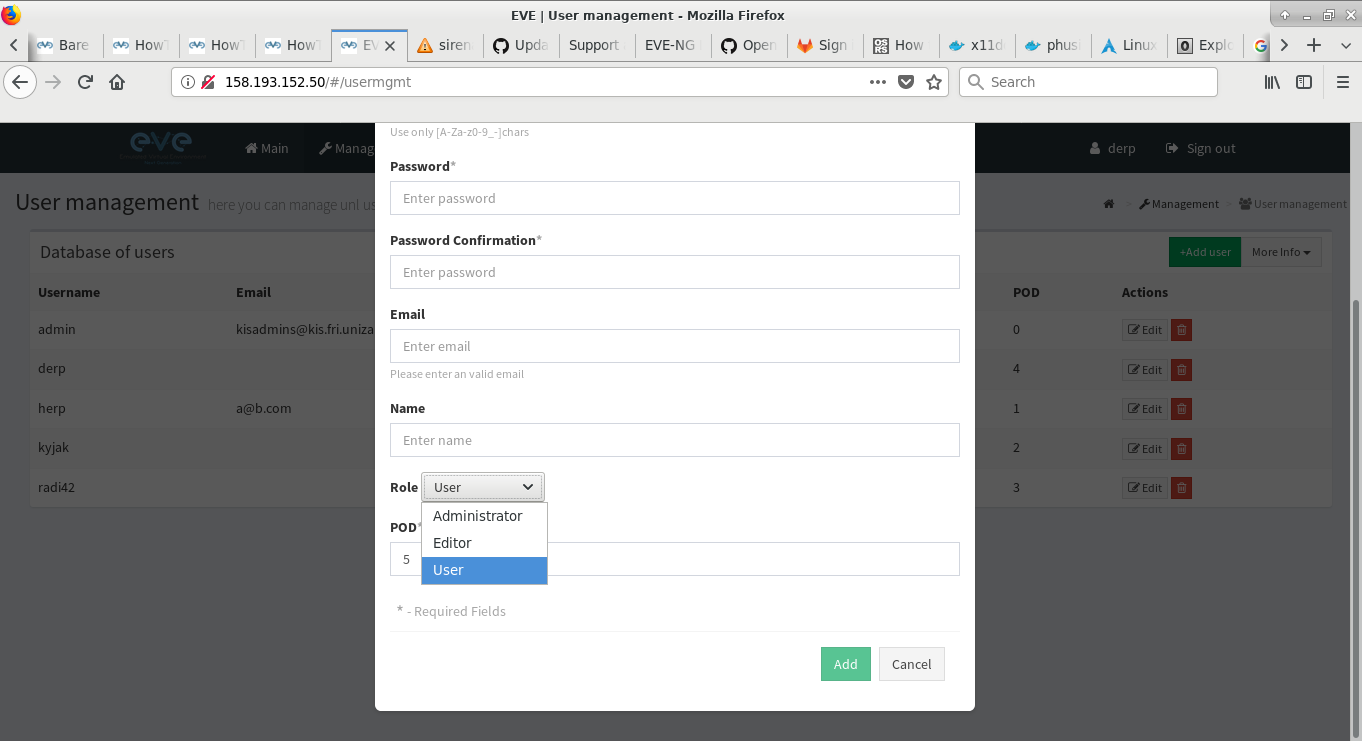
\includegraphics[width=0.75\textwidth]{eve_ng_pouzivatelia_dialog}
    \caption{Dialógové okno na vytvorenie a úpravu používateľa}
    \label{obr:eve_ng_pouzivatelia_dialog}
\end{figure}

Po vytvorení používateľa s inou rolou než \emph{admin}, napr. \emph{user}, sa vo web rozhraní v zozname používateľov stále zobrazujú ako \emph{admin}, hoci v MySQL databázi sú uložení pod správnou rolou v stĺpci \texttt{role} (obrázok \ref{obr:eve_ng_pouzivatelia_mysql}).

\begin{figure}
    \centering
    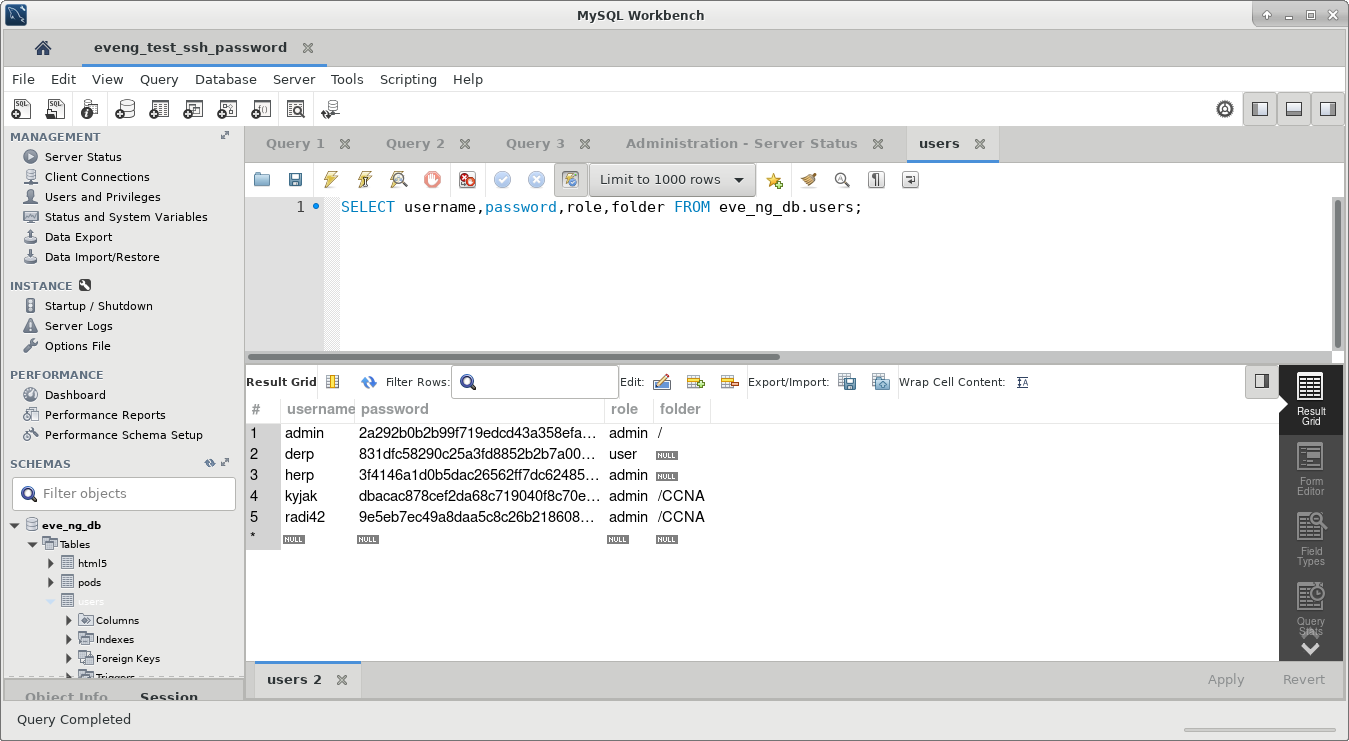
\includegraphics[width=0.75\textwidth]{eve_ng_pouzivatelia_mysql}
    \caption{Zoznam používateľov v MySQL databázi}
    \label{obr:eve_ng_pouzivatelia_mysql}
\end{figure}

Zachytená komunikácia obsahovala aj záznam so správou \\
\texttt{Successfully listed users (60040)} (obrázok \ref{obr:eve_ng_60040}),
ktorej kód sa nachádzal aj v súbore \\
\texttt{/opt/unetlab/html/includes/api\_uusers.php}.

\begin{figure}
    \centering
    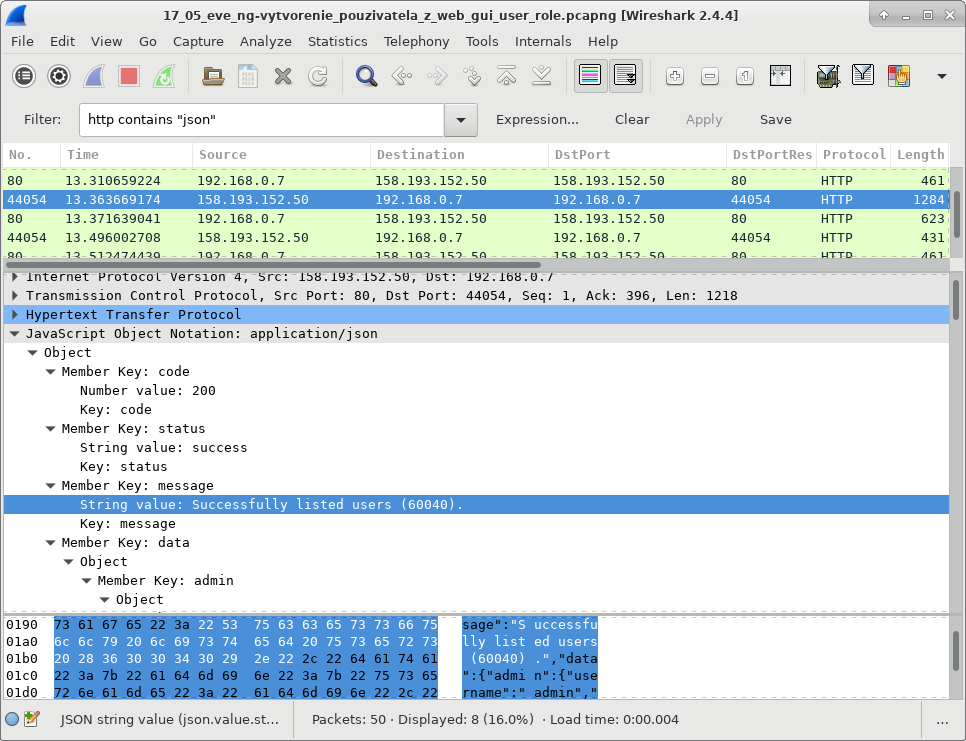
\includegraphics[width=0.75\textwidth]{eve_ng_60040}
    \caption{Správa 60040 - úspešné odoslanie zoznamu používateľov zo servera}
    \label{obr:eve_ng_60040}
\end{figure}

Riešenie spočívalo v úprave funkcii \texttt{apiGetUUser} a \texttt{apiGetUUsers} v spomenutom súbore. Prvá spomenutá funkcia sa stará o získanie informácii o jednom používateľovi, ďalšia o získanie atribútov všetkých používateľov z MySQL databázy. V oboch funkciách sa však vyskytovala rovnaká chyba, a síce, že používateľská rola sa v príkaze \emph{SELECT} napevno prepisovala na rolu \emph{admin}.

Stačilo v týchto príkazoch prepísať názov používateľskej role z pevnej hodnoty \emph{admin} na názov stĺpca používateľskej role t.j. \texttt{role}.

Po vykonanej úprave sa aj vo webovom zozname používateľov zobrazovala ich správna rola (obrázok \ref{obr:eve_ng_pouzivatelia_web}).

\begin{figure}
    \centering
    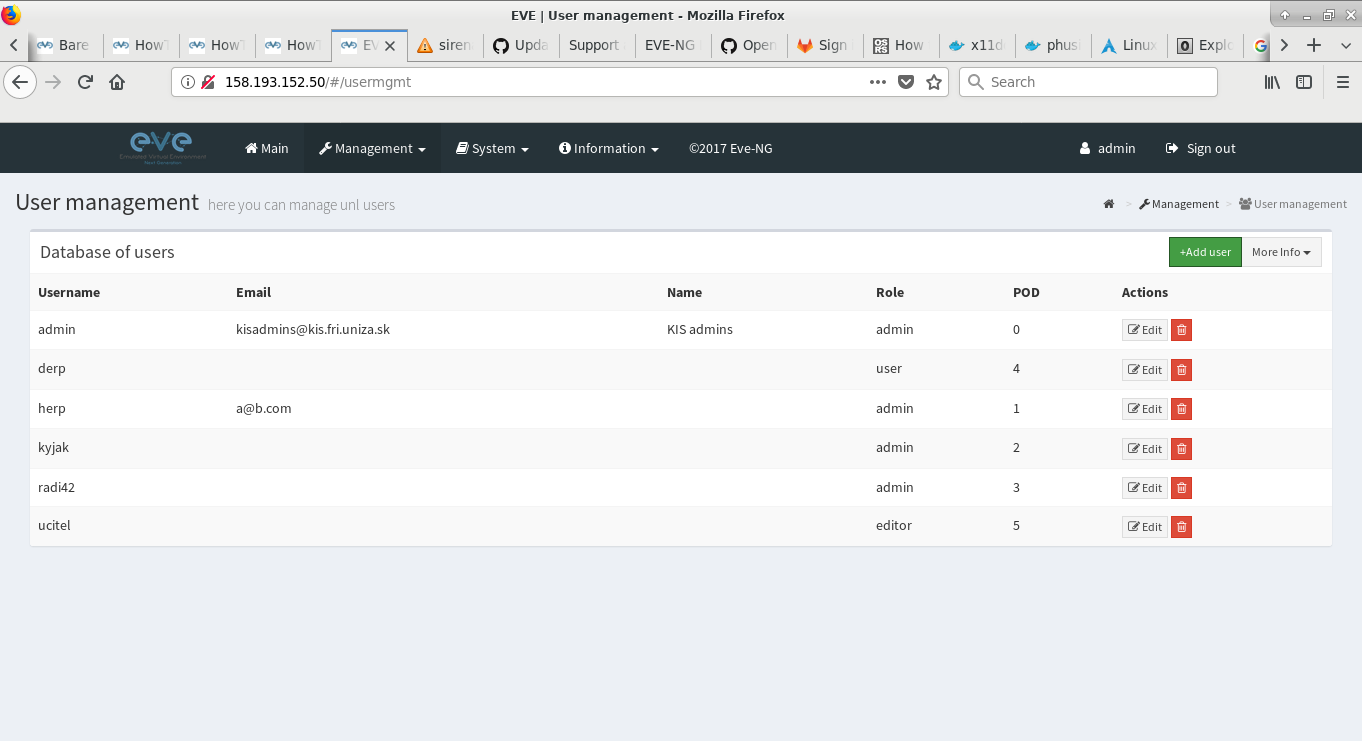
\includegraphics[width=0.75\textwidth]{eve_ng_pouzivatelia_web}
    \caption{Zoznam používateľov vo webovom rozhraní EVE-ng}
    \label{obr:eve_ng_pouzivatelia_web}
\end{figure}

Významom používateľských rolí v EVE-ng sa budeme zaoberať v kapitole \ref{chap:nasadenie_do_vyucovania} - \nameref{chap:nasadenie_do_vyucovania}.




\subsection{Úprava používateľských atribútov}

Atribúty jednotlivých používateľov je možné meniť na obrazovke \emph{User mangement} a môže ich meniť iba používateľ s administrátorskými oprávneniami. Niektoré atribúty, ako sú napr. celé meno používateľa alebo email, sa síce dajú nastaviť, ale následne sa nedajú odstrániť t.j. nastaviť na prázdnu hodnotu. Zmeny sa neprejavia ani vo web rozhraní v zozname používateľov (obrázok \ref{obr:eve_ng_pouzivatelia_web_email_predtym}), ani v MySQL databáze.

\begin{figure}
    \centering
    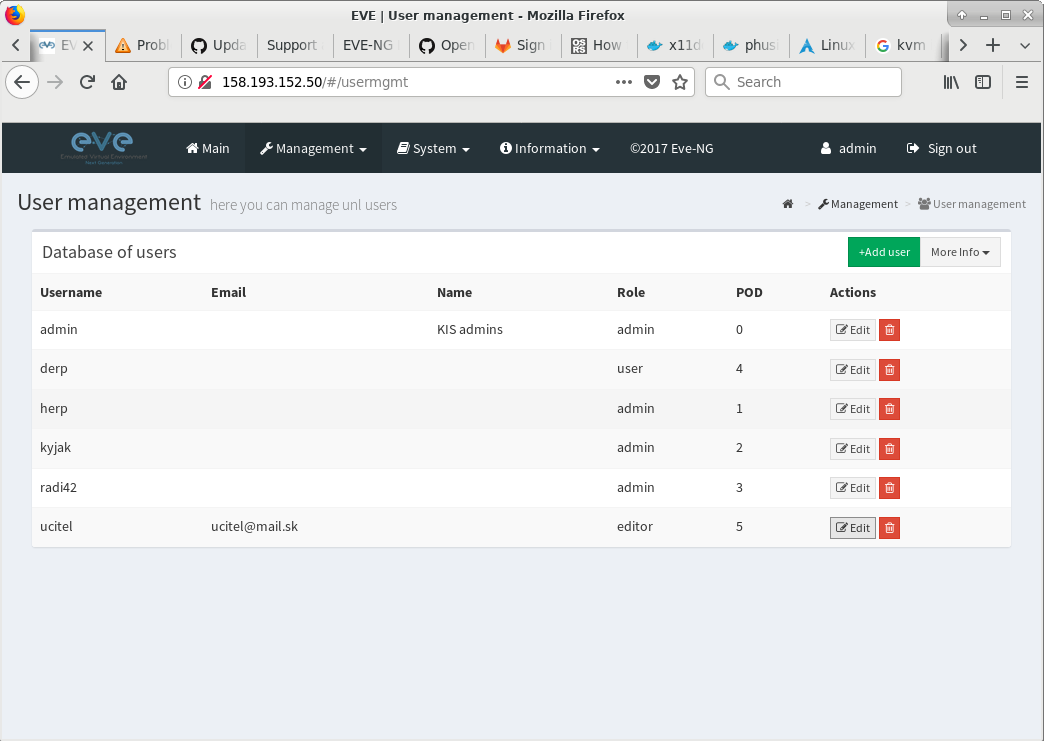
\includegraphics[width=0.75\textwidth]{eve_ng_pouzivatelia_web_email_predtym}
    \caption{Stav pred odstránením e-mail atribútu používateľa \emph{ucitel}}
    \label{obr:eve_ng_pouzivatelia_web_email_predtym}
\end{figure}

Skúsili sme teda odchytiť komunikáciu pri upravovaní spomenutých používateľských atribútov. Zistili sme, po úprave používateľa sa posiela správa \texttt{User saved (60042)} (obrázok \ref{obr:eve_ng_60042}).

\begin{figure}
    \centering
    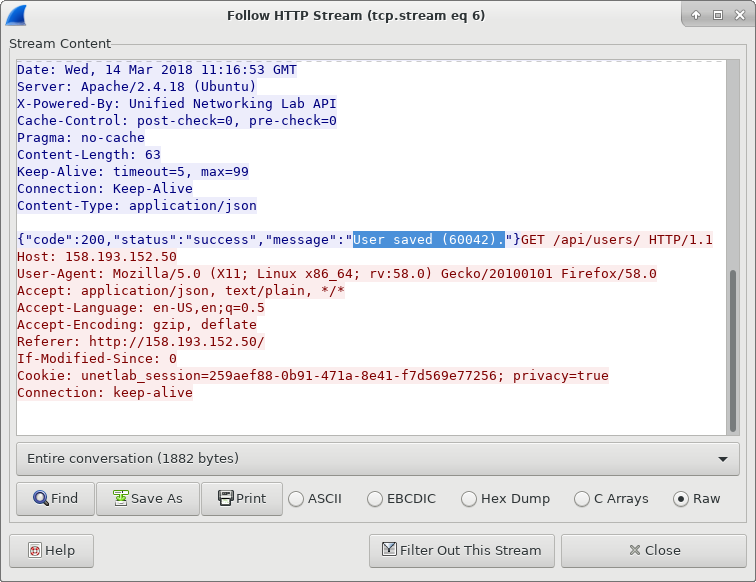
\includegraphics[width=0.75\textwidth]{eve_ng_60042}
    \caption{Správa 60042 - úspešné uloženie atribútov pre používateľa}
    \label{obr:eve_ng_60042}
\end{figure}

Nástroj \emph{grep} ukázal, že kód správy sa vyskytoval o.i. aj v súbore \\
\texttt{/opt/unetlab/html/includes/api\_uusers.php}, konkrétne aj vo funkcii \texttt{apiEditUUser}. Tá ziskava informácie o používateľovi z webového formulára pri úprave tohto používateľa a kontroluje ich správny formát. V prípade, že informácie zadané do webového formulára sú platné, aktualizujú sa atribúty pre konkrétneho používateľa v databáze, v opačnom prípade sa chybne zadané atribúty preskočia.

Problém bol v kontrole vstupov z webového formulára pri úprave používateľa, ktoré boli príliš striktné t.j. nedovoľovali zadať prázdnu hodnotu.

Riešenie spočívalo v upravení kritérii pre atrubúty tak, aby bol aj prázdny reťazec platnou hodnotou.

Po úprave sa už dalo používateľom nielen nastaviť ich celé meno či email, ale aj spomenuté atribúty odstrániť (obrázok \ref{obr:eve_ng_pouzivatelia_web_email_potom}).

\begin{figure}
    \centering
    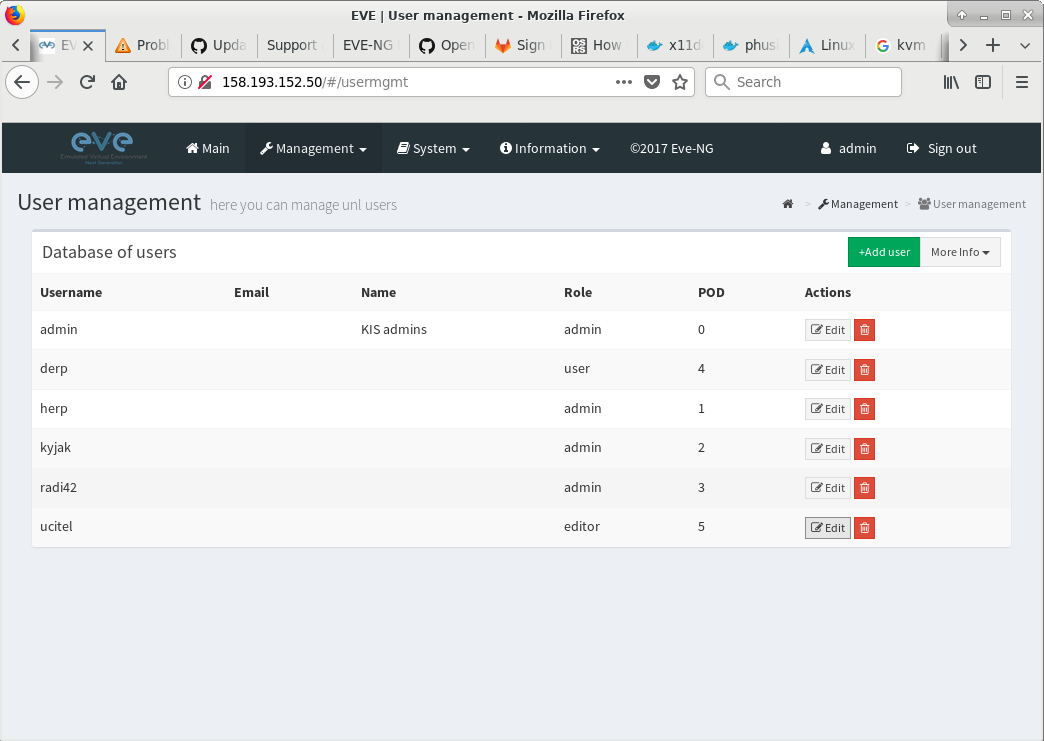
\includegraphics[width=0.75\textwidth]{eve_ng_pouzivatelia_web_email_potom}
    \caption{Zoznam používateľov po odstránení e-mail atribútu pre používateľa \emph{ucitel}}
    \label{obr:eve_ng_pouzivatelia_web_email_potom}
\end{figure}




\subsection{Vypnutie správy o nízkom rozlíšení obrazovky}

Po zmenšení šírky okna približne pod 992 pixelov sa zobrazila správa \\
\texttt{Display too small. This device is not large enough, you need 992px width at least.} (obrázok \ref{obr:eve_ng_display_too_small}).

\begin{figure}
    \centering
    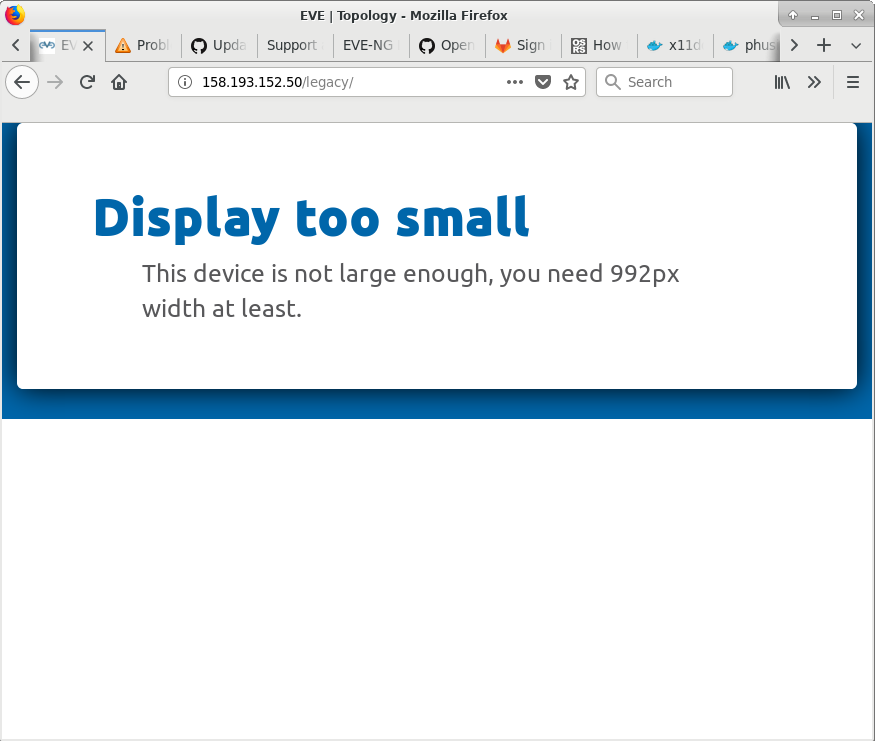
\includegraphics[width=0.75\textwidth]{eve_ng_display_too_small}
    \caption{Chybová správa - \texttt{Display too small.}}
    \label{obr:eve_ng_display_too_small}
\end{figure}

Preto som začal príkazom \emph{grep} hľadať súbory, obsahujúce časti tejto správy. Výstup príkazu obsahoval súbor \\ \texttt{/opt/unetlab/html/themes/default/index.html} \\
ktorý ako jediný obsahoval tento text v nižšie uvedenej časti kódu.

\begin{verbatim}
...
<body>
        <div class="hidden-md hidden-lg container" id="small">
                ...
        </div>
        <div class="hidden-xs hidden-sm container-fluid" id="body">
                ...
        </div>
</body>
...
\end{verbatim}

Skúsili sme zakomentovať všetky riadky v sekcii \texttt{body}, ale následkom tejto zmeny sa stalo otváranie topológii nestabilné a vyskytovali sa rôzne grafické chyby vo vykresľovaní topológie a jej prvkov.

Po experimentovaní so zakomentovaním a upravovaním rôznych riadkov sme našli spôsob, ako túto správu vypnúť. Riešenie spočívalo v zakomentovaní celej sekcie \texttt{div} obsahujúcu atribút \texttt{id="small"} a odstránení tried \texttt{hidden-xs} a \texttt{hidden-sm} z definície sekcie \texttt{div} s atribútom \texttt{id="body"}.

\begin{verbatim}
...
<body>
        <!--<div class="hidden-md hidden-lg container" id="small">
                ...
        </div>-->
        <!--<div class="hidden-xs hidden-sm container-fluid" id="body">-->
        <div class="container-fluid" id="body">
</body>
...
\end{verbatim}

Prvá úprava vypne hlásenie o nízkom rozlíšení obrazovky. Po uložení súboru po prvej úprave a znovunačítaní stránky uvidíme prazdnu bielu obrazovku, ak je okno prehliadača príliš malé t.j. menšie ako približne 992 pixelov.

Druhá úprava odstráni obmedzenie pri vykresľovaní obsahu topológie. Po uložení súboru po prvej úprave a znovunačítaní stránky uvidíme pôvodnú topológiu bez výrazných grafických chýb aj vtedy, ak je okno prehliadača príliš malé t.j. menšie ako približne 992 pixelov.

Po vykonaných úpravách sa problém so zobrazovaním chybovej správy vyriešil, avšak sa vyskytol jeden kozmetický nedostatok. Po zmenšení okna sa zdeformoval posuvník na približovanie a odďaľovanie topológie po zmenšení okna pod kritickú hranicu približne 992 pixelov (obrázok \ref{obr:eve_ng_display_too_small_fixed_but_zoomslider_deformed}).

\begin{figure}
    \centering
    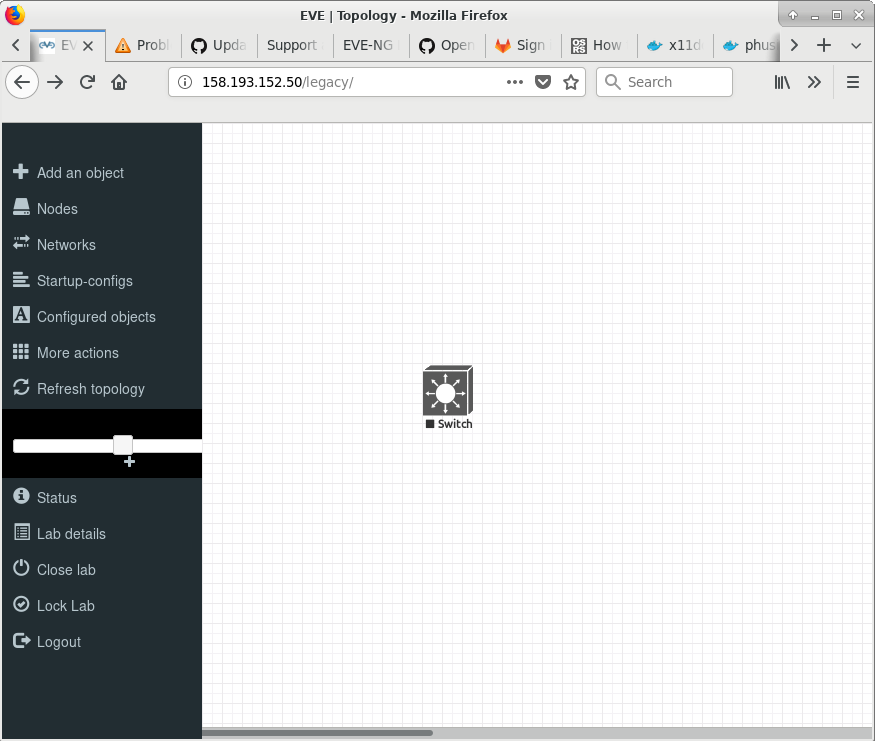
\includegraphics[width=0.75\textwidth]{eve_ng_display_too_small_fixed_but_zoomslider_deformed}
    \caption{Vyriešenie problému s chybovým hlásením \texttt{Display too small.} a deformácia posuvníku na približovanie a odďaľovanie topológie}
    \label{obr:eve_ng_display_too_small_fixed_but_zoomslider_deformed}
\end{figure}

Tento problém sa nám nepodarilo ošetriť. Z "Inšpektora prvkov" vo webovom prehliadači sme zistili, že tento jav môžu spôsobovať napevno zadané hodnoty v súboroch
\begin{verbatim}
/opt/unetlab/html/themes/default/bootstrap/css/bootstrap.min.css
/opt/unetlab/html/themes/adminLTE/build/bootstrap-less/variables.less
\end{verbatim}

Samotný prvok sa volá \texttt{plus-minus-slider} a posuvná plocha sa volá \texttt{zoomslide}, Preto sa riešenie môže skrývať v úprave súborov z výstupu príkazov
\begin{verbatim}
grep -rnw '/opt/unetlab/html/' -e 'plus-minus-slider'
grep -rnw '/opt/unetlab/html/' -e 'zoomslide'
\end{verbatim}

Bol to práve prvok \texttt{zoomslide}, ktorý sa neúmerne zväčšil. Jeho funkčnosť - približovať a oddaľovať prvky v topológii však zostala zachovaná aj napriek tomuto vedľajšiemu účinku.




\subsection{Zatvorenie topológie so spustenými zariadeniami}

Topológiu sa nepodarí zatvoriť, pokiaľ obsahuje spustené zariadenia. Pri zatvorení topológie so spustenými zariadeniami sa vypíše chybové hlásenie \\
\texttt{There are running nodes, you need to power off them before closing the lab.} (obrázok \ref{obr:eve_ng_running_nodes}). \\

\begin{figure}
    \centering
    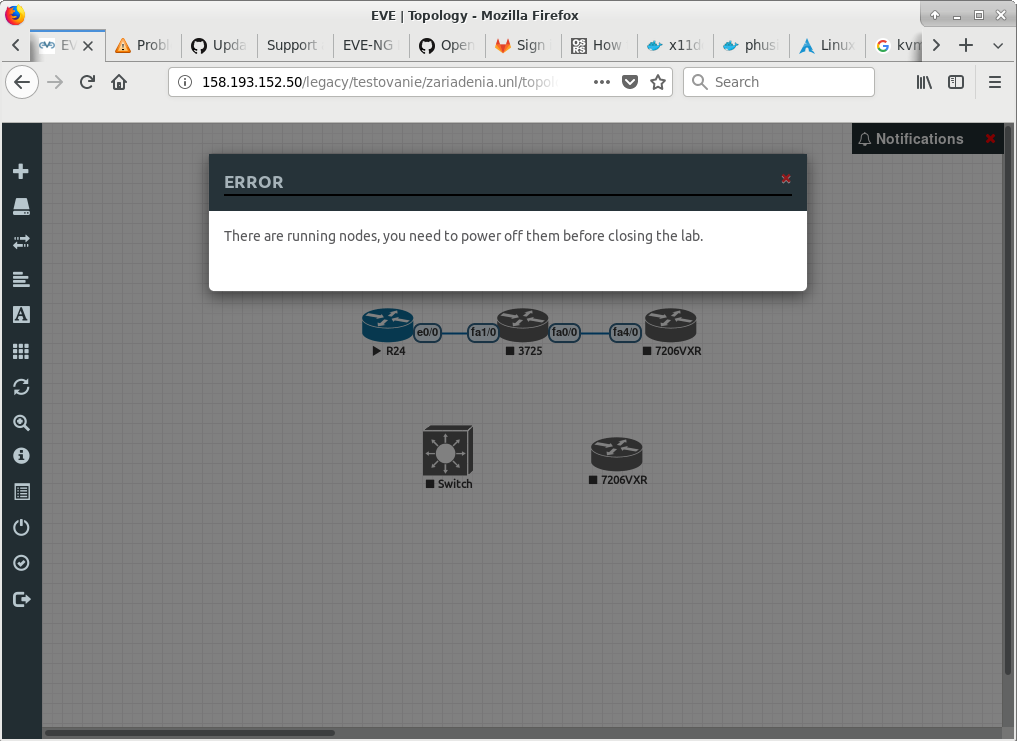
\includegraphics[width=0.75\textwidth]{eve_ng_running_nodes}
    \caption{Chybové hlásenie - topológia so spustenými zariadeniami sa nedá zatvoriť}
    \label{obr:eve_ng_running_nodes}
\end{figure}

Preto sme nástrojom \emph{grep} hľadali, v ktorých súboroch sa vyskytujú časti tejto chybovej správy. Výstup príkazu ukazoval na nižšie uvedené súbory. \\
\begin{verbatim}
/opt/unetlab/html/themes/adminLTE/unl_data/js/angularjs/controllers/lab/labCtrl.js
/opt/unetlab/html/themes/default/js/messages_en.js
\end{verbatim}

Keďže v súbore \texttt{messages\_en.js} sa vyskytujú iba definície chybových hlásení, rozhodoli sme sa upravovať súbor \texttt{labCtrl.js}. V súbore
\begin{verbatim}
/opt/unetlab/html/themes/adminLTE/unl_data/js/angularjs/controllers/lab/labCtrl.js
\end{verbatim}
sa síce táto správa vyskytuje, ale zakomentovanie ľubovoľnej relevantnej časti kódu v metóde \texttt{closeLab} nemá vplyv na funkčnosť t.j. chybové hlásenie sa pri zatvorení topológie napriek tomu zobrazí.

Preto sme sa nakoniec pozreli do súboru \texttt{messages\_en.js}. V ňom bola chybová správa definovaná v poli \texttt{MESSAGES} ako \texttt{MESSAGES[131]}. Znova sa začalo hľadanie výskytov tohto reťazca v súboroch nástrojom \emph{grep}. Výstup príkazu ukazoval na súbory
\begin{verbatim}
/opt/unetlab/html/themes/default/js/functions.js
/opt/unetlab/html/themes/default/js/messages_en.js
\end{verbatim}

Keďže súborom \texttt{messages\_en.js} sme sa už zaoberali, pokračoval som súborom \texttt{functions.js}. V ňom sa vyskytovala aj funkcia \texttt{closeLab}. Tá obsahovala nielen chybové hlásenie, ale aj kontrolu, či v topológii sú už spustené zariadenia. Vypli sme teda túto kontrolu zakomentovaním riadku s podmienkou "if" a celej vetvy "else", ako je uvedené nižšie.
\begin{verbatim}
        //if (running_nodes == false) {
            ...
        //} else {
        //    deferred.reject(MESSAGES[131]);
        //}
\end{verbatim}

Potom sme sa odhlásili, vymazali vyrovnávaciu pamäť webového prehliadača a prihlásili sa do EVE-ng ako používateľ s rolou \texttt{admin}. Potom sme si otvorili súbor s topológiou a pridali do nej niekoľko zariadení. Spustili som zariadenie a pokúsil sa zatvoriť topológiu. Teraz sa chybové hlásenie nezobrazilo a topológia sa úspešne zatvorila. Po znovuotvorení rovnakej topológie zostali zariadenia spustené. Bolo možné aj spustiť ďalšie zariadenia.

Keď sme sa ešte predtým rozhodli riešiť problém so zatváraním topológie so spustenými zariadeniami, skúšali sme v súbore \texttt{functions.js} vo funkcii \texttt{closeLab} zakomentovať celý \texttt{for} cyklus v riadku 
\begin{verbatim}
    $.each(values, function (node_id, node) {
        if (node['status'] > 1) {
            running_nodes = true;
        }
    });
\end{verbatim}
keďže aj v ňom sa nastavovala premenná \texttt{running\_nodes} Po zakomentovaní cyklu sa topológia síce dala zatvoriť aj pri spustených zariadeniach, ale so zariadeniami v nej sa nedalo pracovať napr. nebolo možné zastaviť už spustené zariadenia alebo spustiť ďalšie.

Po opravení tohto nedostatku sa ale vyskytol ďalší problém, ktorý sa odhalil až po vyriešení momentálneho, a síce, že po zatvorení jednej topológie (obrázok \ref{obr:eve_ng_zle_portove_cisla_1}) a otvorení inej (obrázok \ref{obr:eve_ng_zle_portove_cisla_2}) sa zariadenia tvárili, že sú spustené, hoci predtým spustené neboli. Obidva obrázky ukazujú rovnaký počet spustených zariadení v dvoch rôznych topológiách, pričom zariadenia boli spustené iba v topológii na obrázku \ref{obr:eve_ng_zle_portove_cisla_1}. Zariadenia v iných topológiách mali znefunkčnený vzdialený prístup a nešlo s nimi pracovať. Správne fungovali iba tie v pôvodnej topológii. Pokiaľ mali topológie rovnaký počet zariadení a do druhej sme pridali nové zariadenie, toto zariadenie fungovalo bez komplikácii.

Tento jav nastal kvôli tomu, že portové čísla pre jednotlivé zariadenia v topológii sa začínajú číslovať od začiatku rozsahu, ktorý je pridelený danému používateľovi, bez ohľadu na to, ktorá topológia je momentálne otvorená.

Spomenutý problém s rovnakými portovými číslami pre zariadenia v rôznych topológiách sa nám nepodarilo vyriešiť, pretože sa jedná o hlbší problém, ktorého riešenie by znamenalo zmenu mechanizmu na prideľovanie portových čísel v EVE-ng.

\begin{figure}
    \centering
    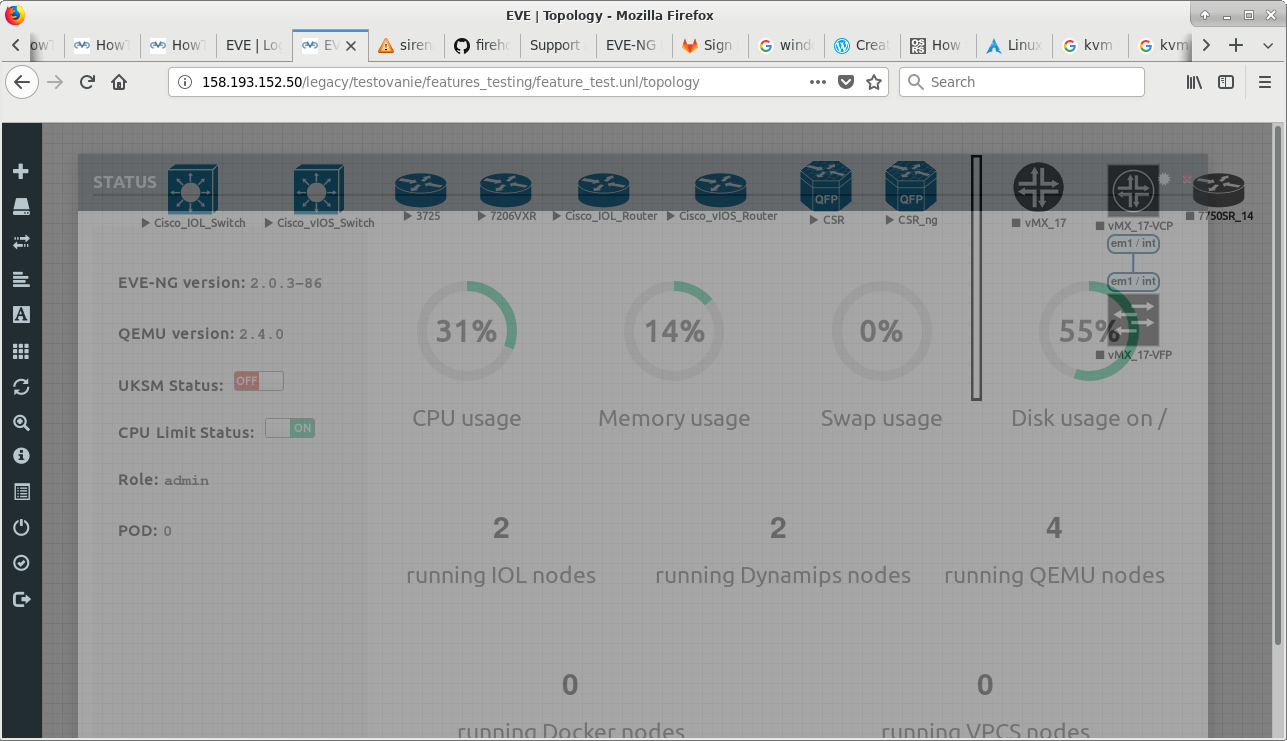
\includegraphics[width=0.75\textwidth]{eve_ng_zle_portove_cisla_1}
    \caption{Prvá topológia a celkový počet spustených zariadení}
    \label{obr:eve_ng_zle_portove_cisla_1}
\end{figure}

\begin{figure}
    \centering
    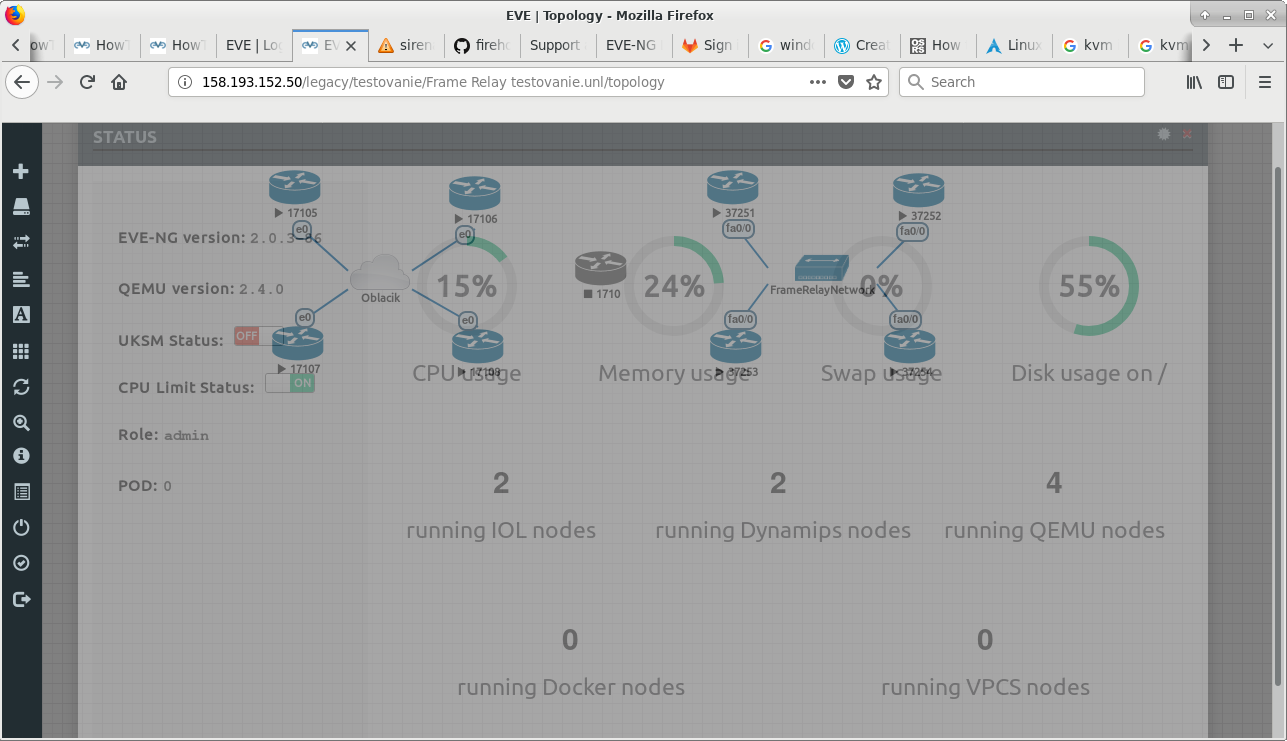
\includegraphics[width=0.75\textwidth]{eve_ng_zle_portove_cisla_2}
    \caption{Druhá topológia a celkový počet spustených zariadení}
    \label{obr:eve_ng_zle_portove_cisla_2}
\end{figure}

Komplikácie, na ktoré sme narazili počas nasadenia na predmety, sú popísané v kapitole \ref{chap:nasadenie_do_vyucovania} - \nameref{chap:nasadenie_do_vyucovania}.




\section{Administrácia}

EVE-ng server je vytvorený tak, aby sa po jeho konfigurácii bolo potrebné oň starať čo najmenej. V nasledujúcich častiach budú opísané veci súvisiace s jeho administráciou.




\subsection{Adresárova štruktúra}
\label{chap:adresarova_struktura}

Tu je uvedený krátky zoznam najdôležitejších adresárov v EVE-ng. Podrobnejší zoznam súborov a adresárov sa nachádza v dokumentácii na priloženom CD.

\begin{longtabu} to \textwidth {| X[3.0,l,m] | X[4.0,l,m] |}
\caption{Adresárová štrukúra EVE-ng servera}
\label{tab:adresare} \\
\hline
    \multicolumn{1}{|c|}{\textbf{Adresár}} & \multicolumn{1}{|c|}{\textbf{Popis}} \\
\hline
    \texttt{/opt/unetlab/addons/} & \makecell[lc]{Adresár obsahujúci všetky zariadenia, \\ ktoré je možné pridať do topológie. \\ Obsahuje podadresáre \texttt{dynamips}, \texttt{iol} a \texttt{qemu}, \\ podľa toho, pre aký typ hypervízora je zariadenie \\ určené - Dynamips, IOL alebo QEMU/KVM} \\
\hline
    \texttt{/opt/unetlab/addons/iol/bin/} & \makecell[lc]{Adresár s Cisco IOL zariadeniami spolu s \\ vygenerovanou IOL licenciou} \\
\hline
    \texttt{/opt/unetlab/addons/iol/lib/} & \makecell[lc]{Adresár s Cisco IOL ovládačom potrebným \\ na spustenie Cisco IOL zariadenia} \\
\hline
    \texttt{/opt/unetlab/html/templates/} & Šablóny pre každý typ zariadenia v topológii \\
\hline
    \texttt{/opt/unetlab/data/Logs} & Súbory o zázname činností na serveri \\
\hline
\end{longtabu}




\subsection{Zálohovanie}
\label{chap:zalohovanie}

Kritické súbory a adresáre sú automatizovane zálohované nástrojmi \emph{cron} a \emph{rsync}. Pre tento účel bol vytvorený skript, ktorý používa nástroj \emph{rsync}. Ten synchronizuje adresáre a súbory len vtedy, pokiaľ zistí, že sa majú nahradiť novšími verziami. Nástroj \emph{cron} je nastavený tak, že vykonáva tento skript každý deň počas noci, kedy sa na serveri vyskytuje minimálna aktivita.




\subsection{Monitorovanie}

Monitorovanie systému je dôležitým prostriedkom v prípade, že zaznamenáme nižšiu výkonnosť servera. Na monitorovanie systémových zdrojov EVE-ng servera môžeme, okrem tradičného nástroja \emph{htop} použiť aj vstavaný nástroj na monitorovanie systémových zdrojov vo webovom rozhraní EVE-ng.

Vstavaný monitorovací systém EVE-ng sa nachádza vo webovom rozhraní v časti \emph{System} -> \emph{System status}. Rovnaký panel je prístupný aj z rozhrania topológie v menu na ľavej strane obrazovky po kliknutí na položku \emph{Status}. Zobrazuje prehľad o aktuálnom percentuálnom vyťažení procesora, operačnej pamäte a diskového priestoru spolu s celkovým počtom spustených zariadení každého druhu. Nástroj je znázornený na obrázku \ref{obr:eve_ng_system_status}.

\begin{figure}
    \centering
    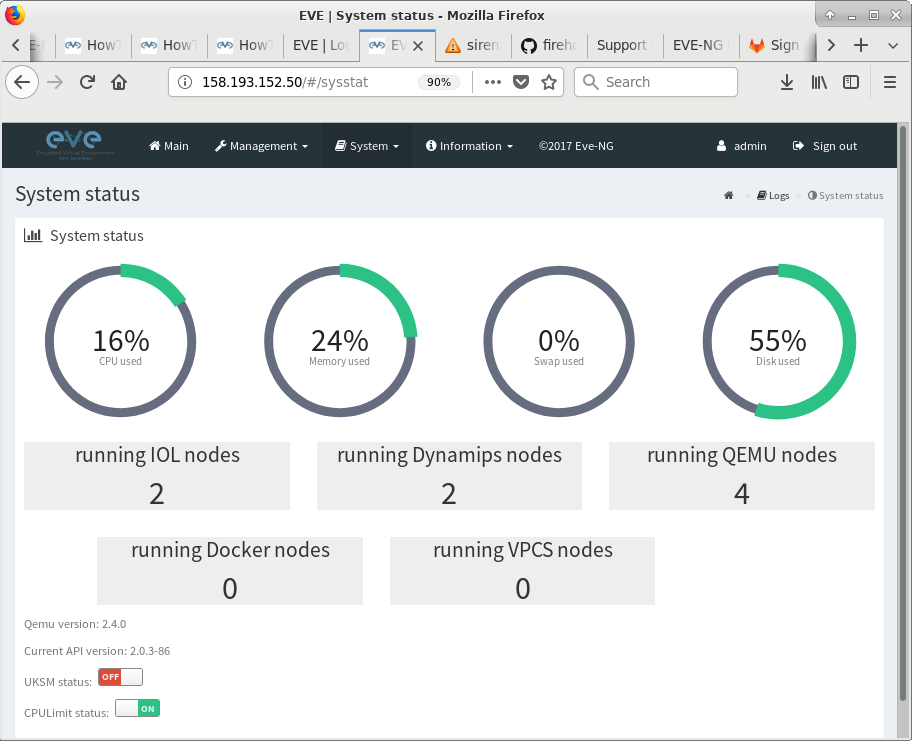
\includegraphics[width=0.75\textwidth]{eve_ng_system_status}
    \caption{Monitorovanie systému vo webovom rozhraní EVE-ng}
    \label{obr:eve_ng_system_status}
\end{figure}




\subsection{Správa používateľov EVE-ng}

{\huge TODO - Kde sú uložení používatelia - v MySQL databáze}

Zoznam používateľov webového rozhrania v EVE-ng je znázornený na obrázku \ref{obr:eve_ng_pouzivatelia_web_email_potom} (str. \pageref{obr:eve_ng_pouzivatelia_web_email_potom}). Obrazovka sa nazýva \emph{User management} a je prístupná z horného menu kliknutím na \emph{Management} -> \emph{User management}. Pre každého používateľa sú definované nasledujúce stĺpce:

\begin{itemize}[noitemsep]
    \item \textbf{Username} - Používateľské meno. Používa sa na prihlásenie sa do webového rozhrania. Musí byť unikátne pre každého používateľa.
    \item \textbf{Email} - Emailová adresa.
    \item \textbf{Name} - Celé meno používateľa. Atribút má iba informatívny charakter.
    \item \textbf{Role} - Používateľská rola. Definuje oprávnenia prihláseného používateľa.
    \item \textbf{POD} - Identifikačné číslo používateľa. Určuje rozsah portov, ktoré sa používajú na vzdialený prístup ku zariadeniam v topológii. Musí byť unikátne pre každého používateľa.
    \item \textbf{Actions} - Úprava atribútov používateľa (Edit) a odstránenie používateľa (Delete). Po kliknutí na tlačidlo \emph{Edit} v riadku vybraného používateľa sa otvorí dialógové okno na vytvorenie a úpravu používateľa zobrazené na obrázku \ref{obr:eve_ng_pouzivatelia_dialog} (str. \pageref{obr:eve_ng_pouzivatelia_dialog}).
\end{itemize}

Dialógové okno na vytvorenie a úpravu používateľa sa zobrazí po kliknutí na tlačidlá \emph{Add user} a \emph{Edit}. Pozostáva z týchto častí:

\begin{itemize}[noitemsep]
    \item User Name
    \item Password
    \item Password Confirmation
    \item Email
    \item Name
    \item Role
    \item POD
\end{itemize}

Všetky polia majú rovnaký význam ako v popise stĺpcov na obrazovke so zoznamom používateľov. Novým prvkom sú polia \emph{Password} a \emph{Password Confirmation}. Tie nie je nutné vypĺňať, ak ich nechceme meniť. Ak chceme používateľovi heslo zmeniť, je potrebné zadať nové heslo do obidvoch polí. Na zmenu hesla na nové nie je nutné zadávať pôvodné heslo. Pole \emph{User Name} sa pri úprave používateľa nedá zmeniť, dá sa iba jednorázovo nastaviť pri vytváraní používateľa. Pole \emph{POD} je vyplnené automaticky najnižším voľným identifikátorom.

Ak sme vykonali kroky v časti \ref{chap:eve_ng_pouzivatelske_role} - \nameref{chap:eve_ng_pouzivatelske_role}, budú po kliknutí na rozbaľovací zoznam pre atribút \emph{Role} dostupné, okrem role \emph{admin}, aj role \emph{editor} a \emph{user}. Tieto role sa medzi sebou líšia oprávneniami na výkon určitých činností. Zoznam činností pre každú používateľskú rolu je popísaný v nižšie uvedených zoznamoch.

\noindent
Zoznam úloh, ktoré môže vykonávať používateľ s rolou \emph{user}:

\begin{itemize}[noitemsep]
    \item Prehliadať súbory a adresáre
    \item Prehliadať topológiu
\end{itemize}

\noindent
Zoznam úloh, ktoré môže vykonávať používateľ s rolou \emph{editor}:

\begin{itemize}[noitemsep]
    \item Všetko, čo môže vykonávať používateľ s rolou \emph{user}
    \item Spravovať súbory a adresáre - vytváranie, presúvanie, premenovanie, odstránenie
    \item Upravovať prvky v topológii - pridávanie, presúvanie, premenovanie, odstránenie
    \item Upravovať vybrané atribúty používateľov - meno, email
    \item Exportovať/importovať súbory s topológiami
    \item Zamknúť topológiu, aby bola pre používateľov typu \emph{user} iba na čítanie
\end{itemize}

\noindent
Zoznam úloh, ktoré môže vykonávať používateľ s rolou \emph{admin}:

\begin{itemize}[noitemsep]
    \item Všetko, čo môže vykonávať používateľ s rolou "editor"
    \item Zastaviť všetky zariadenia v "System -> Stop All Nodes"
    \item Zobraziť informácie o konkrétnom používateľovi cez API
    \item Spravovať všetkých používateľov - pridať, upraviť, odstrániť
    \item Zapnúť/vypnúť UKSM v "System -> System status"
    \item Zapnúť/vypnúť KSM v "System -> System status", ak je KSM dostupné
    \item Zapnúť/vypnúť CPULimit v "System -> System status"
    \item Aktualizovať EVE-ng z web rozhrania cez koncový bod "/api/update" v UNetLab/EVE-ng API
\end{itemize}

Niektoré z týchto činností nie sú implementované vo webovom rozhraní EVE-ng. Činnosti, ktoré môžu vykonávať jednotlivé používateľské role sú definované v súbore "/opt/unetlab/html/api.php". Vyznačujú ich riadky

\begin{verbatim}
  ...
  if (!in_array($user['role'], Array('admin'))) {
  ...

resp.

  ...
  if (!in_array($user['role'], Array('admin', 'editor'))) {
  ...
\end{verbatim}

Vyššie uvedené podmienky kontrolujú, či je používateľ s danou rolou oprávnený vykonať požadovanú operáciu. Napr. vytvoriť používateľa, premenovať adresár, presunúť súbory do adresára a pod.

V prípade, že používateľ nemá dostatočné oprávnenia sa zobrazí chybové hlásenie \texttt{Not enough access privileges for this operation (90032)}, ktoré znázornené na obrázku \ref{obr:not_enough_access_privileges}.

\begin{figure}
    \centering
    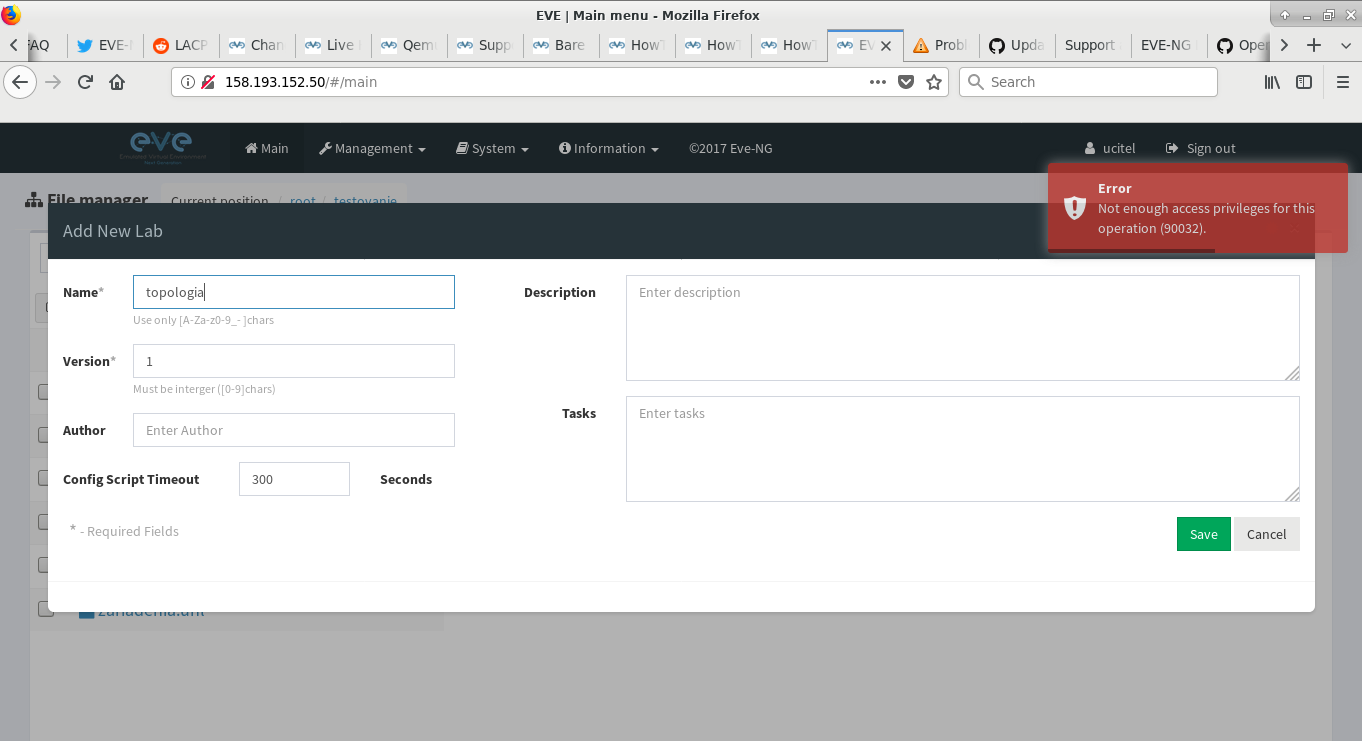
\includegraphics[width=0.75\textwidth]{not_enough_access_privileges}
    \caption{Chybové hlásenie o nedostatočných oprávneniach používateľa}
    \label{obr:not_enough_access_privileges}
\end{figure}

Niekedy sa však táto správa pri vykonaní neoprávnenej činnosti nezobrazí, čo ale nemá žiadny vplyv na funkcionalitu a daná operácia sa nevykoná.